\documentclass[12pt]{report}

%%\usepackage{setspace}
\usepackage{amsfonts}
\usepackage{amsmath}
\usepackage{amssymb}
\usepackage{amsthm}
\usepackage{enumerate}
\usepackage{mathrsfs}
\usepackage{alltt}
\usepackage{color}
\usepackage{fancyvrb} 
\usepackage{graphicx}
\usepackage{epstopdf}
\usepackage{url}
\usepackage{verbatim}
\usepackage{hyperref}
%\usepackage[autostyle]{csquotes} 
%\usepackage[toc,page]{appendix}

\usepackage[top=1in, bottom=1.5in, left=1.5in,right=1.5in]{geometry} % setting the page alignment with this package

\DeclareGraphicsExtensions{.png}

\hypersetup{
    colorlinks=true, %set true if you want colored links
    linktoc=all,     %set to all if you want both sections and subsections linked
    linkcolor=black,  %choose some color if you want links to stand out
    citecolor=black
}

\begin{document}

\begin{titlepage}
\begin{center}
\thispagestyle{empty}
% TODO maybe nice pic? \includegraphics [width = 0.3\textwidth] {images/wpilogo}\\[0.3cm]
% TODO install \textsc font
\Large{\textbf{A Major Qualifying Project Report\\ \large{ON}}}\\[0.7cm]
\LARGE{\textsc {\textbf{An Analysis of the Feasibility and Performance of BitTorrent as a Data Transfer Protocol in Peer to Peer Backup Systems}}}\\[0.5cm]
\vspace{0.2cm}
\Large{\textbf{\\Submitted to the Faculty of }}
\LARGE{\textbf{\\WORCESTER POLYTECHNIC INSTITUTE\\}}
\vspace{0.5cm}
\Large{\textbf{\\In Partial Fulfillment of the Requirement for the}}
\Large{\textbf{\\Degree of Bachelor of Science}}
\vspace{0.5cm}
\Large{\textbf{\\by}}\\[0.5cm]
\large{\textbf{Dan Bouffard}}\\
\large{\textbf{Marc Green}}\\
\vspace{0.5cm}
\large{\textbf{UNDER THE GUIDANCE OF}}\\
\large{\textbf{Professor G\'abor N. S\'ark\"ozy}}\\
\vspace{1cm}
\large{\textbf{\\May 1, 2014}}\\
\end{center}
\end{titlepage}

\begin{abstract}
Abstract
\end{abstract}

\renewcommand{\abstractname}{Acknowledgements}
\begin{abstract}
Acknowledgements
\end{abstract}

\tableofcontents
\listoffigures

\chapter{Introduction}

Introduction


\chapter{Background}
\section{Centralized Backup Systems}
% TODO: get reliable sources for number of users of OneDrive and Google Drive
Several popular backup systems currently in use have a centralized system design. In these systems, there are many clients that all back up their data to a central location controlled by a single entity. Common elements of these systems include a fixed amount of data storage per person, with the option to obtain more for a fee. Three of the more popular systems are Dropbox, which has over 200 million users \cite{dropboxusers}, OneDrive, with over 250 million users, and Google Drive, with over 120 million users.

There are several benefits to using a centralized backup system. The first is that it is very probable that the service will always be on, as the content is being stored on servers dedicated to that purpose. Companies who offer file backup services have the hardware resources to store redundant copies of data, should a server fail. They will also have the personnel to investigate and fix any problems with the service.

However, there are also several problems with using a centralized system to back up data. One of these problems is that there is a single point of failure, should the storage site be compromised in some way (for example, natural disasters). This is less of a problem for big companies with the resources to handle these situations, but there is still a cost to take the necessary preventative measures when creating the system.

Another problem with centralized systems is a matter of trust: when a user stores his or her data using a third party, the third party essentially has control of that data. Even if the third party claims to offer encryption for all data that they hold, there could still be a backdoor in the service that allows them or another entity to obtain an unencrypted version of the data. One solution to help combat this is to manually encrypt the data before sending it to the third party, but this is hardly a convenient solution.

% TODO: reliable sources for data caps and monthly/yearly fees
Finally, there are often restrictions on what can be stored using centralized backup systems. This includes both the size of individual files and the amount of total data. More space is gained by paying a monthly or yearly fee, but even then the amount of space is capped at a specific size. For users who need to back up a large amount of large files, these systems are not very useful.

Peer to peer backup systems, on the other hand, provide an equivalent service and suffer from none of these drawbacks. 

\section{Peer to Peer Backup Systems}

Peer to Peer (P2P) Backup Systems are applications that allow users to back up data without the use of a central entity. Instead, each user offers some of his or her storage space in order to use the space of others as backup locations. We start this section by introducing peer to peer networks, and then discuss the technical components of existing P2P backup systems.

\subsection{Peer to Peer Networks}

A peer to peer network is a type of distributed network model in which participants form direct connections to each other. This is in contrast to the centralized client-server network model, in which all participating clients connect to a central server to carry out their task. Client-server network models are used on the World Wide Web: the clients are users' web browsers and the server is the website being visited. In peer to peer networks, each participant, or "peer", functions as both a client and a server; peers initiating a request take on the role of the client, and peers answering the request take on the role of the server.

In the client-server model, servers are expected to always be available and accessible. Peer to peer networks do not have this luxury. Instead, they experience the constant fluctuation of peers joining and leaving the network. This is called \textit{churn} \cite{StorageSearchP2PNetworks}. Churn in P2P networks complicates the communication between peers because the sought peer may be offline. This is especially a problem in P2P backup systems; for example, a peer might try to recover data from another peer who is not online. The strategies for dealing with churn, and many other P2P-specific complications, heavily depend on the type of overlay network a P2P application uses. We discuss churn in more detail in section \ref{sec:churn}.

% TODO add reference for p2p explanation/definition

\subsubsection{Overlay Networks}

An overlay network is any network built on top of another network. That is, an overlay network consists of nodes with neighbors who are not physically connected, but instead use the underlying network to establish a virtual connection. They need not be constrained by the limitations of the physical world. Consider a trivial example where there are three computers connected to the Internet, but located in different parts of the world. These three computers could form an overlay network by agreeing to be virtual neighbors to each other. If their overlay network was used in a P2P application, then, when connecting to each other, they will use the underlying network, the Internet, to actually send messages. The P2P application does not need to know about the underlying network that is used to route messages; it only needs to know that there is an overlay network that defines the direct connections between peers.

Peer to peer applications use overlay networks as their foundation.\footnote{Overlay networks are used for many purposes, not just P2P applications. Note, however, in discussing overlay networks, we will still refer to their participants as \textit{peers}.}  The P2P overlay network provides structure for the application that uses it, allowing peers to find each other.

There are three categories of overlay networks that can be used as the network abstraction on which a P2P network is built. \textit{Structured} overlay networks organize peers according to some geometry, e.g., a ring. This structure is strictly maintained as nodes join and leave the network. \textit{Unstructured} overlay networks, on the other hand, do not organize peers, but instead allow the network to grow into any shape, determined only by the routing table of each peer. \textit{Hierarchical} overlay networks are composed of multiple groups of peers each forming their own overlay network. A representative peer from each group joins a top-level overlay network, connecting the distinct groups \cite{p2pSurvey}. 

We discuss structured overlay networks in more detail below, as that is the type of overlay network our P2P backup system uses.

\subsubsection{Structured Overlay Networks} \label{subsubsec:StructuredOverlayNetworks}

Structured overlay networks are defined by a topology and a virtual address space. For example, in our system, peers are organized in a ring and addressed by 20 byte numbers---our address space is the set of all 20 byte numbers. In other systems, peers could be organized in a 3D cube and addressed by their (x,y,z) coordinates. The topology defines the set of neighbors each peer has in the overlay. The address space serves as a way to uniquely identify peers.
% TODO maybe insert figure of chord ring topology (or our own!)

The purpose of peer to peer networks (and more broadly, networks in general) is to share data. In the P2P networks that focus not just on sharing data, but also storing, locating, and possibly retrieving data (like ours), the data shares the same virtual address space as the peers. That is, these structured overlay networks give the data themselves valid addresses. For example, in our system, the data being backed up is also given a 20 byte "address". This is done to determine which peer is responsible for a given piece of data. Specifically, a peer is responsible for all data in the address space that the peer is closest to. It is for this reason that peer address assignment should be evenly distributed, to keep the distribution of work equal. Aside: the average size of the address space for which a peer is responsible decreases as more peers join the network, which allows these types of networks to easily scale in size.

To join a structured overlay network, a peer must know at least one other peer already in the network. This peer is often called the \textit{bootstrap peer}. The joining peer will contact the bootstrap peer to find its proper place in the topology. We come back to this below in more detail in our explanation of how to find other peers.

% TODO cite router.bittorrent.com as well known bootstrap node?
%In BitTorrent's structured overlay network \footnote{To clarify, we are referring to BitTorrent's distributed hash table, not its unstructured network. The latter involves using centralized trackers, the former removes such dependency. We refraim from using the term \textit{distributed hash table} to keep the explanation simple without loss of generality. We discuss distributed hash tables in section \ref{sec:backgroundDHT}.}, a well known bootstrap node \footnote{The BitTorrent specification uses \textit{node} to refer to participants of its structured overlay network and \textit{peer} as a more general term \cite{bittorrentDHT}. We will adopt this convention when speaking about BitTorrent, and use them interchangeably otherwise.} is router.bittorrent.com. A BitTorrent node randomly chooses a 160 bit \textit{nodeID} to use as an address. To join the network, it will contact a bootstrap node to find the nodes it is closest to in the topology. Closeness, in BitTorrent's case, is determined by taking the $XOR$ of \textit{nodeID}s; smaller values are defined as closer \cite{bittorrentDHT}.
% TODO define XOR?
% TODO maybe remove this entire paragraph, since it doesn't really clarify anything. it just gives another example of picking an id and mysteriously finding nodes its closest to. if we end up remove it, we should reword end of previous paragraph
% TODO maybe keep it in b/c we refer to closness in 3.1.1

Leaving a structured overlay network can be as simple as not responding to any messages. Our system, like many others, leaves this functionality undefined. Node failures due to hard shutdowns will not follow the protocol to leave the network, so it is easiest to treat all node departures as node failures. 

To find other peers, a peer in a structured overlay network will consult its routing table. This table is initially populated upon joining the network, and is kept up to date as peers join and leave. When a joining peer first contacts a bootstrap peer, it is unlikely that the bootstrap peer has the joining peer's direct neighbors in its routing table. This is because the routing table is designed to include many peers that are close, and only a few peers that are far\footnote{This is to provide an efficient, $O(\log n)$ time complexity. This means that given n nodes, it will take less than $c \times \log n$ steps (for some $c$), which is good performance.} A joining peer, by asking the bootstrap node, will learn of the peers in the bootstrap peer's routing table that the joining node is close to. The joining peer will then contact these peers, ask for the same information, and learn of peers it is even closer to. This process repeats until the joining node learns its direct neighbors \cite{p2pSurvey}.

Overlay networks are the abstraction that connects all the users of a P2P system. It is the foundation on which a P2P application can be built, and is responsible for providing methods for peers to join and leave the network, and find other peers in the network. Furthermore, structured overlay networks allow the P2P application to locate specific information very quickly because their virtual address space provides full accountability of any piece of data. It is for this reason we chose a structured overlay network as the substrate of our P2P application; it is easy to determine which peer is responsible for a given backup because we know it will be the one closest in the address space.\footnote{However, churn complicates this. For example, a peer with an even closer address may join the network between storing and retrieving the data.}

% TODO may need better segue between p2p networks and file chunking

% TODO: Ask Sarkozy/Mihaly if they think keeping this section in is worth it.
\subsection{File Chunking} \label{sec:filechunking}
The format in which files are stored can have an effect on the efficiency of the P2P backup system. At first, backing up each file as a whole might seem like the obvious choice, since files are only useful in their entirety. However, the creators of the P2P backup systems pStore \cite{pStore} and PeerStore \cite{PeerStore} have shown that there are benefits to splitting files up into chunks, rather than distributing complete files to peers. In these systems, this is accomplished by creating two types of files: a "file block", which contains a section of the original file, and a "file block list", which contains information on which file blocks compose the original file and how to order them. This has the benefit of having data units be a fixed size that will be easy to store for any node. For example, if a peer needs to store a 10GB file, it does not need to find a peer capable of storing 10GB (which might be rare); rather, it needs to find $file\_size/chunk\_size \times number\_of\_replicas$ peers. Although lowering the chunk size will increase the chances of finding a peer to store on, it is important to choose a reasonable chunk size, as using more nodes for storage will add more overhead in finding those nodes.

File chunking also gives the benefit of easy versioning and updating of files. When a newer version of a file is backed up, the only chunks that need to be reinserted into the network are the ones that differ from the previous version. Old versions of file chunks stay in the network, so that any full version of the file can be reconstructed by requesting the appropriate file chunks. Backup systems can also reduce the amount of storage space used by sharing identical file chunks between peers.

Our system does not use file chunking. Instead, by using BitTorrent as the data transport protocol, we have applied the concept of splitting files into chunks in a new way in P2P backup systems. We distribute complete files to each backup location, but separate files into chunks when they are being transferred; this is how BitTorrent works. With the BitTorrent Protocol, a peer can download a file by requesting chunks of it from many peers at the same time. By utilizing the upload bandwidth of several peers, a file can be downloaded quicker than if it were directly downloaded from one entity (see section \ref{sec:TheBitTorrentProtocol} for more details).

\subsection{Fairness} \label{sec:BackgroundFairness}
Another aspect of P2P backup systems is fairness between peers. Peers need to be storing an amount of data proportional to the amount that they are backing up to other peers. This can be challenging to enforce, because untrustworthy peers can attempt to game the system to obtain free backup storage. For example, consider a simple system where each peer must offer to store the same amount of data that they back up on other peers. A peer could claim that all of the storage space that it should be offering is being used by other peers, while in reality the peer has not taken in any other peer's data. It is clear that a mechanism needs to be built into the system that ensures that peers store the data of each other.

PeerStore handles this via a combined trading and challenge system. When a peer wants to create a backup of its data, it finds a peer to trade data with. In its request to back up data, the peer will also advertise that it is willing to store a certain amount of data for its trading partner. The peer that receives the request will then need to accept or reject it, and if the request is accepted, the acceptor will also need to request a certain amount of storage in return. If the original requestor accepts this offer, then the two become trading partners and will send each other data. This process is illustrated in figure \ref{fig:peerStoreTrading} \cite{PeerStore}.

\begin{figure}
  \centering
  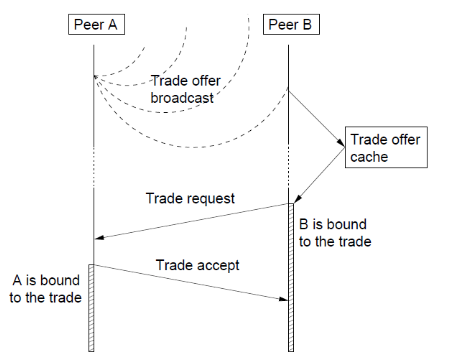
\includegraphics[scale=0.75]{PeerStoreTrading}
  \caption{Trading protocol of PeerStore \cite{PeerStore}}
  \label{fig:peerStoreTrading}
\end{figure}

While this ensures that peers will agree to take data in proportion to the amount that they want to back up, it still does not guarantee that peers hold onto that data. For example, a peer could form a trading agreement with another peer, exchange data, and promptly discard the received data. To combat this, peers can periodically challenge each other to prove that they are actually storing data. This is the approach that we, like PeerStore, propose. We provide peers the ability to ask each other to prove they are storing the data that they are supposed to be storing. A peer proves itself by replying with a value that could only be derived if they were, indeed, safekeeping the data. See \ref{subsec:ChallengeMechanism_sec:Fairness_chap:BTBackup}
 for more details about our proposed challenge mechanism.

\subsection{Churn and Data Migration} \label{sec:churn}
With each storage node being regular users, it is often the case that nodes can be offline. Recall that churn refers to the fact that peers will continuously enter and leave the P2P network. The designer of a P2P backup system must take this into consideration if the system is to provide reliable access to backed up data. This has been accomplished via data migration \cite{pStore,PeerStore}, where the availability of files is periodically checked and replicas are made when the peers being used for backup are not reliably available. Other data migration algorithms have been designed specifically to work in high churn networks \cite{StorageSearchP2PNetworks}. In this case, data replicas are periodically redistributed to different groups of nodes, which means that newer nodes have a chance to store data. This is beneficial because data stays evenly distributed throughout the overlay network, preventing any single node from being responsible for too much data, regardless of when they joined.\footnote{It is important to note this strategy is designed to work in an unstructured overlay network, not a structured one. Structured networks need not redistribute like this because the evenly distributed address assignment provides the even data distribution.}

The number of replicas to maintain will have an impact on the performance of the system. If the replica count is too low, the probability of recovering the  file is lowered. If the replica count is too high, then storage space and bandwidth will be needlessly used. Furthermore, if the system requires a peer to offer a proportional amount of storage space to the amount that it is using on others, the peer will also have to offer a lot more space than what it is using locally for its own data. % TODO this last sentence might go better in the fairness section 

\subsection{Cryptography} \label{sec:crypto}
Crytography is the study of techniques for secure communication in the presence of third parties \cite{cryptoDef}. It is heavily relied upon in the computer world to protect secrets, verify identities, and ensure data hasn't been tampered with. Our system uses cryptography to \textit{encrypt} users' data before replicating it to stranger's computers. Encryption is the process of obfuscating text into a state such that it cannot be understood without reversing the process. There are several types of encryption proccesses, each with its respective \textit{decryption} process. Decryption refers to reversing the encryption so that encrypted message becomes readable again.

In \textit{symmetric key cryptography}, the encryption and decryption processes use identical \textit{keys}. The key is the secret parameter to the mathematical functions that prevents anyone else from decrypting the data. Anyone who has the key for a given message can decrypt it. Using a different key to encrypt the same data will result in a different output.

Encryption in P2P backup systems is necessary to prevent the peers who are storing backups of data from reading it. A system in which backups were unencrypted would be much less popular with users, because they would lose privacy by using it. The terminology associated with this is \textit{confidentiality}, meaning that data that is supposed to be confidential, remains confidential.

\textit{Hashing} is the process of applying a \textit{hash function}, which uses a mathematical function, to some arbitrary-length message, resulting in a fixed sized \textit{hash}. Regardless of the input, the hash will usually look like a random string of characters because the mathematical function manipulates the underlying data. This manipulation greatly changes the bits originally used to represent the input data. A good hash function will uniformly distribute the hashes it produces to minimize \textit{collisions}. Collisions are when two inputs hash to the same value, and are often undesired, especially in \textit{cryptographic hash functions}. Cryptographic hash functions are hash functions that are suitable for use in cryptography. They possess mathematical properties that allow for confidentiality to be provided, among other properties.

To strengthen hashing algorithms, a \textit{salt} can be utilized. A salt is essentially a randomly picked string of bytes that is concatenated to data to be hashed. The use of different salts with the same sequence of data creates a different hash (since the total input the hash function is different). The same hash will be calculated if the same salt is used with the same sequence of data. Using salts is a useful technique in preventing \textit{dictionary attacks}, where an attacker compares a precomputed list of inputs and their hashes with a target hash of some unknown data in an attempt to find out what the unknown data is. Dictionary attacks are common on password hashes, because, upon success, the attacker will discover the password used to generate the password hash. With a salt, the precomputed hash for the data wll not match. The list of hashes cannot be easily recomputed with the salt, since hashing is designed to be an expensive and lengthy operation.

\textit{Convergent encryption} is a technique used in pStore and PeerStore to ensure confidentiality \cite{pStore, PeerStore}. Convergent encryption involves taking the hash of the unencrypted data, and then using the hash as the symmetric key to encrypt the data. The main benefit of using convergent encryption is that the same data will be encrypted the same way each time, so identical blocks in the network can be shared between peers in their encrypted form, without the need for a complicated key exchange protocol. Convergent encryption is illustrated in figure \ref{fig:convergent}.

\begin{figure} \label{fig:convergent}
  \centering
  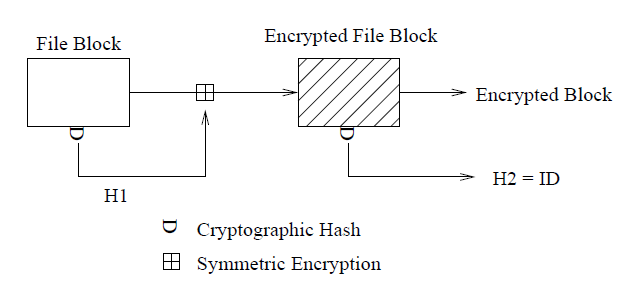
\includegraphics[scale=0.75]{ConvergentEncryption}
  \caption{Convergent Encryption from PeerStore}
\end{figure}

While this is a convenient optimization, it has a security weakness: any user who has access to the unencrypted version of a file can confirm whether or not that file is being stored in the system. This encroaches on users' privacy.

% TODO relate convergent encryption to our system

\section{Distributed Hash Tables} \label{sec:backgroundDHT}

A \textit{hash table} is a data structure that maps unique keys to values. It has attractive performance features, such as $O(1)$ average lookup time. This means that, on average, the time it takes to retrieve a value from the hash table is independent of the number of entries being stored. This performace comes from the use of a hash function when organizing the data internally, the details of which is out of the scope of this paper. Hash tables also have $O(1)$ insertion and deletion time.

A \textit{distributed hash table} (DHT) is a hash table that is stored across mutliple nodes. Each node is responsible for a portion of the hash table's contents. In exchange for distributing the storage cost among several nodes, DHTs do not have $O(1)$ search, insertion, or deletion time. However, this is generally acceptable because the usefulness of distributing the storage cost far outweighs the drawback of slower operations on the data structure. This is especially true since the network latency will likely overshadow the slower performance of the data structure. The alternative would be to have each peer keep a copy of the entire hash table. This solution suffers from several problems: it makes the hash table hard to maintain, the download time can become nontrivial, and it might become infeasible to store the entire table on regulars peers, since it can become huge with larger networks.

% TODO discuss DHTs being good with churn, scale well

% TODO citations?


DHTs play a major role in many P2P systems. They serve as the means through which peers can find either data or other peers, depending on the system; our system uses a DHT for the latter. In conjunction with the structured overlay network, the DHT allows for peers to discover each other. This is primarily done when looking for peers to send backups to. We discuss how we use a DHT in more detail in section \ref{sec:DataExchange}.

\section{The BitTorrent Protocol} \label{sec:TheBitTorrentProtocol}
BitTorrent is a peer to peer protocol designed for fast file sharing. A peer who wishes to share a file creates a .torrent file containing metadata about the file to be shared. This peer is known as the file's initial \textit{seeder}, or uploader, and through the use of a BitTorrent client, starts \textit{seeding}, or uploading, the file. When a peer acts as a seeder, its sole purpose is to share the file that it is seeding with other peers. Peers who wish to download the file must acquire its .torrent file through an out-of-band channel, which is often a torrent indexer. Peers use the .torrent file to locate the initial seeder through either a centralized tracker or a DHT. These peers then connect to the initial seeder and start downloading the file. These peers are known as \textit{leechers} until they possess a full copy of the file, which is when they, themselves, become seeders.

% TODO: add citation and more information about how much better BitTorrent is vs. direct download. Actually, add a lot of citations to this paragraph
While this is more complex than hosting a file on a server and having users download it, with enough peers there is a huge performance gain with respect to download speeds. The reason this works is due to the differences in upload and download speeds on the Internet; with most Internet connections offered to consumers, the upload bandwidth is much smaller than the download bandwidth. This means that, in the scenario where one machine is tranferring data over the Internet to another machine, download speeds would be severely limited by the upload bandwidth of the uploader. If multiple machines are trying to download from the same uploader, the download speeds will be even worse, as the upload bandwidth is being shared.

% TODO: finish this paragraph
The BitTorrent Protocol takes advantage of this by having leechers download content from multiple peers who are a part of the torrent. A file is partitioned into several \textit{chunks}, or file blocks, and a file download is performed by requesting these chunks from multiple peers. % Use combined upload bandwidth, etc.

BitTorrent can transfer files quickly due to multiple seeders each uploading different chunks of the file to each leecher. This parallelized download is enhanced by the fact that leechers, too, upload the chunks of the file they possess to other leechers who do not have those chunks. \footnote {This is a simplified version of the BitTorrent protocol. For more information, see \cite{bittorrentProtocol}}

\section{BitTorrent Sync}
BitTorrent Sync is a new application developed by BitTorrent, Inc. It is a P2P synchronization tool that allows users to share files between trusted devices. This is accomplished by generating a set of 20-byte "secrets" for each folder to share and distributing the secret to each trusted device. All data is encrypted using AES-128 in counter mode \cite{btsynctech}, the key of which is derived from the secret. There are three different secrets, each of which provide different permissions for the peer that is given the secret: the read/write secret, the read only secret, and the encryption secret, which allows the node to store an encrypted version of the data so that it cannot read the contents. A variation of the read/write and read only secrets also exists called the one-time secret, which allows a peer to send out a valid key that is only usable by one node \cite{btsyncuserguide}.

Users of BitTorrent Sync have several options for having their synced devices locate each other. The following list is taken from the BitTorrent Sync technology page \cite{btsynctech} and describes each method of peer discovery:

% TODO why do we discuss the different ways to find peers? We only need to talk about predfined hosts
\begin{quote}
\begin{itemize}
\item Local peer discovery. All peers inside local network are discovered by sending broadcast packets. If there are peers with the same secret they respond to the broadcast message and connect.
\item Peer exchange (PEX). When two peers are connected, they exchange information about other peers they know.
\item Known hosts (folder settings). If you have a known host with a static ip:port, you can specify this in Sync client, so that it connects to the peer using this information.
\item DHT. Sync uses DHT to distribute information about itself and obtain the information about other peers with this secret. Sync sends SHA1(Secret):ip:port to DHT to announce itself and will get a list of peers by asking DHT for the following key SHA1(Secret)
\item BitTorrent tracker. BitTorrent Sync can use a specific tracker server to facilitate peer discovery. The tracker server sees the combination of SHA1(secret):ip:port and helps peers connect directly. The BitTorrent Sync tracker also acts like a STUN server and can help do a NAT traversal for peers so that they can establish a direct connection even behind a NAT.
\end{itemize}
\end{quote}

To allow other developers to use BitTorrent Sync as a part of their applications, the BitTorrent Sync API has been created \cite{btsyncapi}. Developers can obtain an API key by applying for one and have the application accepted by the BitTorrent Sync developers. The API key allows a developer to use all API functions, which are issued in the form of HTTP requests sent to the web interface that is started by the BitTorrent Sync executable.

BitTorrent Sync leverages the BitTorrent protocol to provide quick downloads between synced peers. We, too, leverage this through the use of BitTorrent Sync to provide fast recovery of backed up files. The specification of our system is described in the next chapter.

\chapter{BTBackup}

In this chapter, we discuss the design of our Peer to Peer backup system. See Chapter \ref{chap:impl} for our implementation of it.

\section{Data Exchange} \label{sec:DataExchange}

% todo reword
This section discusses the infrastructure and the protocols of our system that are concerned with moving data between entities in the network. Henceforth, we use the following terminology to disambiguate participants:

% todo use package enumitem to make labels italics instead of bold
\begin{description}
  \item[Peer:] A particpant who is sending replicas of their data into the network for safekeeping. We refer to this process as \textit{backing up} data.
  \item[Node:] A participant who is storing a replica for a peer. We refer to this process as \textit{storing} data.
\end{description}
  
This terminology is used to give context. It is very likely that every participant in the system will eventually serve both roles (perhaps even simultaneously), but we refer to them as \textit{peer} or \textit{node} depending on what role they are playing in a given situation. A peer plays the role of the client, whereas a node plays the role of a server.\footnote{We may qualify each term to help give context. For example, we may say "\ldots a \textit{replication} node \ldots" to emphasize the fact that the node is storing a replica.} When there is no context, we use the terms interchangeably. 
% TODO find/replace all uses of replicant node with replication node or vice versa

Note the emphasis of the action taken by each: a peer is said to \textit{back up} data, and a node is said to \textit{store} a replica of the peer's data. 

PeerStore showed that separating the metadata layer from the data layer can result in significant bandwidth reduction. By relaxing the requirement to strictly maintain a set number of replicas per file, the system can reduce the data migration cost. For example, it is unneccessary to immediately find a new replication node when a current replication node goes offline; only when the node has shown to be consistently unavailable should the system seek a replacement. Given that there exists more than one replica of a peer's data, having one temporarily offline is not catastrophic.\footnote{Note that this implies the low possibility of not being able to recover data that is backed up. Note that this situation is unavoidable in \textbf{all} backup systems. By relaxing the aforementioned requirement like PeerStore, we leverage this fact by sacrificing theoretical availability for performance and usability. See section \ref{subsec:TheMetadataLayer_sec:SystemDesign} for the discussion of the parameterization of these variables in our implementation. See section \ref{} for our methodology of testing the parameter. Finally, see section \ref{} for a comparison of the results of different values for the parameter.}
% TODO add references once we know section names

Our system separates the two layers as well: the metadata layer is responsible for storing information about each data layer exchange (among other information), and the data layer is responsible for the actual exchange of the data.

\subsection{The Metadata Layer} \label{sec:TheMetadataLayer_DataExchange}

In the broadest sense, the metadata layer is used by peers to find nodes. Peers use it to determine which nodes will be used to store their data, and, in the event of local data loss, peers use it to find those same nodes so they can recover their data. The former is described below in \textbf{Finding Replicant Nodes}, the latter in \textbf{Metadata Record}.
% TODO don't hardcode these

The metadata layer is a DHT that maps a given \textit{node ID} to information about the node (e.g., its IP address), called its \textit{metadata record}. A \textit{node ID} is a unique identifier for a node. It is used as the address of the node in the structured overlay network.

\subsubsection{Metadata Record} \label{subsubsec:MetadataRecord}

A \textit{metadata record} is used for three purposes:

\begin{enumerate}
  \item Find the IP address of the node it describes
  \item Determine if the node it describes should be used to store one's data 
  \item Find the nodes to which the peer it describes is backing up\footnote{To clarify: each metadata record belongs to single entity. In the first two use cases, a peer looking to back up data queries for the node's metadata record. In the last use case, a peer starts the data recovery process by querying for its own metadata record. The entity requesting the metadata record (and the reason for doing so) changes based on the context.}
\end{enumerate}

A metadata record stores the following information for each node in the system: (node IP, blacklisters, backed up files, stored files). A thorough explanation of the information stored in a metadata record follows. Table \ref{tab:metadataRecord} summarizes the information.

\begin{description}
  \item[Node IP:] The IP address of the node that the metadata record describes. This is used by peers who wish to back up a file on this node to directly contact it.
  \item[Blacklisters:] The list of (peer ID, timestamp) pairs, where the peer IDs are the IDs of those who have determined that the node is \textit{unreliable} (see section \ref{sec:ChurnandDataMigration_DataExchange} for the definition of what makes a node unreliable) and the timestamp is the time when the ID was inserted. This information is used by peers who are considering using the node as a backup location. If the node has too many blacklisters (greater than some number $n$), peers will decide against using that node, and move on to select another node. In order to prevent sybil attacks, where a malicious user has many identities and blacklists a node many times, $n$ should be a nontrivial amount and proportional to the size of the network. In order to prevent nodes from permanently being shut out from the network, entries in the blacklist are removed some set amount of time after they are inserted; this is accomplished via the aforementioned timestamp.
  \item[Backed Up Files:] The list of information on the files backed up by the peer that the metadata record describes. Each element in the list stores the following data: the \textit{file ID}, the filesize, the list of replication node IPs, and a timestamp indicating when each replication node stored the file. The file ID is a unique identifier for the file, and must be in the same address space as node IDs (as explained in section \ref{subsubsec:StructuredOverlayNetworks}). This information is used by peers looking to recover their data. After retrieving their own metadata record, peers will ask the corresponding replication nodes to transfer the data for each file they wish to recover. The more replication nodes that are online for a given file, the faster the recovery of the file (due to the BitTorrent protocol used in the data layer). The timestamp is not yet used, but is included because future revisions to the specification may need it (for example, for peers to check that the node's replica is up-to-date).
  \item[Stored Files:] The list of information on the files stored by the node that the metadata record describes. Each element in the list stores the following data: the file ID, the filesize, the peer backing up the file, and a timestamp indicating when the node stored the file. This information, in conjunction with the information in \textbf{Backed Up Files}, is used as part of the fairness mechanism, described in section \ref{sec:Fairness}.
\end{description}

\begin{table}
\begin{center}
    \begin{tabular}{| l | l |} 
    \hline
    Node IP & The most recent IP address used by this node\\ \hline
    Blacklisters & List of peers who consider this node unreliable\\ \hline
    Backed Up Files & List of information on files this peer has backed up \\ \hline
    Stored Files & List of information on files this node stores for other peers \\ \hline
    \end{tabular}
    \caption{Summary of a metadata record}
    \label{tab:metadataRecord}
\end{center}
\end{table}

\subsubsection{Finding Replicant Nodes} \label{subsubsec:FindingReplicantNodes}

For every file a peer wishes to back up, it must find a predetermined number of nodes that can store the file. To ensure an even distribution of responsibility in the structured overlay network, a random bitstring in the address space of the overlay network is generated; the DHT provides the functionality to find the node whose ID is \textit{closest} to the randomly generated bitstring, for the overlay network's given definition of closeness. The peer then gets the metadata record for the candidate node from the DHT. From the metadata record, the peer can calculate if the candidate node is \textit{obligated} to store its file. We discuss the situation in which a node is obligated to store a peers file in section \ref{sec:Fairness}. The peer also uses the metadata record to ensure the candidate node does not have too many blacklisters. If the candidate node meets both requirements, the peer chooses it to store a replica and uses the data layer to contact the node to inform it of the decision. The metadata layer is updated appropriately, and the data layer is used to transfer the file. This process repeats until the predetermined number of nodes are found.

\subsection{The Data Layer} \label{subsec:TheDataLayer}

The data layer is responsible for copying the data to be backed up from the peer to the node. This includes the quick communication by the peer to the node informing it that it is a replication node for a given file.

Our main contribution in this paper, and the only requirement of the data layer, is that it uses BitTorrent as the data transport protocol. By doing so we increase the speed of data recovery, because the peer can download the data from all replication nodes simultaneously.

\subsubsection{Security}

The data that is transported via the data layer is encrypted so that the replication nodes cannot read it. The strength of the encryption is left unspecified as a means of future-proofing this specification.

% TODO note that this isn't done in the impl
Furthermore, all communication between peers and nodes is encrypted to limit information leakage.

\subsection{Churn and Data Migration} \label{sec:ChurnandDataMigration_DataExchange}

%If less than X number of replicas, a peer should make a new replica on a node that has yet to hold a replica. (is this a TODO?)
For users of our system to take advantage of the speed increases offered by the BitTorrent protocol, a sufficient number of replicas need to be maintained in the overlay network (for a comprehensive explanation of how the BitTorrent protocol works, see section \ref{sec:TheBitTorrentProtocol}). Since the P2P network will be composed of ordinary network users, backups that are created may not always be available. Therefore, it is not enough to rely on the backups that are created when a file is first backed up; in the worst-case scenario, all of the nodes on which a user has created replicas have permanently left the network, leaving the user with no way to retrieve any backup. If one or two replication nodes are online when the backups are needed, the user will be able to recover their file but will not see much of a speed benefit from the BitTorrent protocol, as opposed to when all replication nodes are online.

To solve this problem, peers in our system periodically check on the nodes that they are using as backup locations in order to gauge how available they are. During normal program operation, each peer tests the availability of its replication nodes via a challenge mechanism, described in section \ref{subsec:ChallengeMechanism_sec:Fairness_chap:BTBackup}. The challenge mechanism not only ensures the node is online, but also confirms it is storing the peer's data. If the replication node is online and passes the challenge, the peer does not need to do anything; it will continue to (accurately) think that the node is reliable. If the node fails the challenge (by being offline or not storing the user's data), however, the peer will take note that the node was unreliable in this instance. It would be unfair to immediately conclude that the node is consistently unreliable, since it may have been temporarily offline (for example, a user temporarily shutting down his/her computer). Therefore, a node needs to fail the challenge mechanism several times before the peer concludes that it is consistently unreliable. It is possible that a node gets unlucky and happens to be offline during all checks, even though it is online during a different part of the day. If this is the case, then the node is not frequently available for that peer, and should be seen as consistently unreliable from the peer's perspective.

When a peer determines that a node is consistently unreliable, it does two things. The first is that it adds its own ID to the node's blacklist in the DHT. The second is to move its replica to a new node. The peer sends an update to the DHT that it is removing the replica on the unreliable node. This accomplishes two things: all other peers in the network can see that the node is storing less data, and the node can see that it no longer needs to store the replica, so it can remove it the next time it checks the DHT for any changes. The peer will then look for a new node to put a replica on, using the same process that was used for creating the original backups (see section \ref{subsec:TheMetadataLayer_sec:SystemDesign}). Since this process uses a randomly generated salt to help pick the ID of the new node, each node has an equal chance of being selected, assuming that it has enough space to store the replica and is not blacklisted by too many peers. This helps to prevent some nodes from being left out of the selection process. % TODO this last sentence can be removed without loss of information, but it might mean that the salt explanation in the crypto section was for nothing.

\section{Fairness} \label{sec:Fairness}
% People store proportional amount of data compared to how much they are backing up
% TODO we say "if n backups", but also refer to each backup as a "replica". we should be consistent. where else do we do this? ctrl-f replica
To ensure fairness (see section \ref{sec:BackgroundFairness} for background information), each node must contribute storage space proportional to the amount that they are backing up. Since a peer will have replicas of its file stored on multiple nodes, the amount of space that a peer offers\footnote{That is, offers to store when it assumes the role of a node} must be much larger than the amount of unique data that it is backing up. If $n$ backups are maintained for each file and $F$ represents the set of files that a peer backs up, the total amount of space $t$ that the peer must offer can be expressed as:
\begin{equation}
t=n\sum\limits_{i=1}^{|F|} size(F_i)
\end{equation}
There exists one problem with this mechanism: when the network first starts up, no peer has created any backups, so no one is obligated to store data for other peers. To solve this, our system requires that each peer is obligated to take at least $s$ bytes of data from other peers, regardless of how much data it has backed up. To include this, $t$ can be reexpressed as:
\begin{equation}
t=max(s,n\sum\limits_{i=1}^{|F|} size(F_i))
\end{equation}
When a peer finds a node that has a value of $t$ greater than the size of the file it is trying to replicate, it can choose that node as a replication site, knowing that it will be able to accept the data.

\subsection{Challenge Mechanism} \label{subsec:ChallengeMechanism_sec:Fairness_chap:BTBackup}
Even though the technique described above allows peers to find nodes with a sufficient amount of storage space, it does not guarantee that the node will keep its promise and actually store the data. For instance, a node can accept a peer's data, only to discard it immediately. A peer will only find out that its data has been discarded when it needs to retrieve backups, at which point it is too late to create new backups.

To combat this, we have designed a challenge system that forces nodes to prove that they are actually storing the data that they are claiming to store. This system is based on the mechanism used in PeerStore \cite{PeerStore}. A challenge in our system consists of a randomly-generated salt followed by a specified range of bytes in the file being backed up. The node holding the peer's data must take the bytes in the specified range, hash it using the provided salt, and return the result to the peer. The peer is able to test whether the answer is correct by encrypting the file in the same way as it is stored on the node and hashing the byte range accordingly. If the correct answer is returned, then the node has passed the challenge. If the node does not respond or gives the wrong answer, the challenge has been failed. By choosing a random subset of bytes and by using a salt, the node cannot calculate the hash ahead of time and only store that; the whole file must be stored in order to be able to successfully complete all possible challenges.


\chapter{Implementation} \label{chap:impl}

Our goals for the implementation of BTBackup were to make it a fast, modular, platform independent system that is as close to the specification as time permitted. Furthermore, it should allow us to adequately analyze the feasibility and performance of BitTorrent Sync as the data transport protocol in the backup system.

\section{Language and Tools}

Our implementation of BTBackup is written in C++. This language was primarily chosen for its speed. We use the Boost library (version 1.55) to remain platform independent. We use Jsoncpp (version 0.6.0-rc2) to serialize and unserialize the JSON that the implementation uses for message passing. We use cURLpp (version 0.7.3) to interface with the BitTorrent Sync Web API.

\section{System Design}
\subsection{Overview} \label{subsec:Overview_sec:SystemDesign_chap:Implementation}
%Diagram of system design
We have designed our system to be modular. We realize that future work on our system might include the replacement of our data and metadata layers. Our solution for making these parts interchangeable with different implementations is to define standard interfaces between the two layers and the core application. These interfaces can be followed to create new implementations for the two layers. Along with these two layers, there is one more major part to our application: the system core. The system core comprises the core functionality of our system, which includes accepting and executing user commands, receiving network requests from other peers, and maintaining the P2P system.

\begin{figure} \label{fig:SystemDesign}
  \centering
  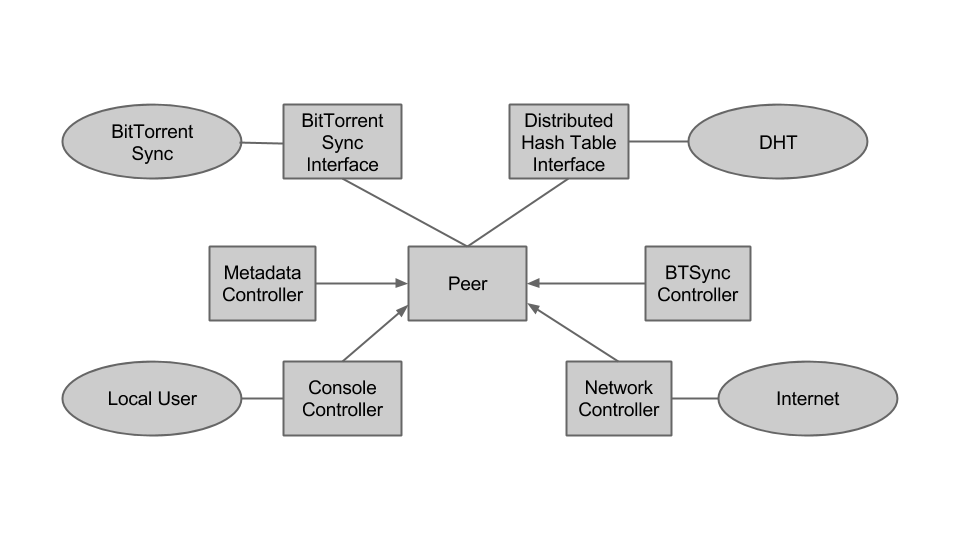
\includegraphics[scale=0.4]{SystemDesign}
  \caption{The design of our system}
\end{figure}

We explain each of these components in the following sections.

\subsection{The Data Layer}
% TODO: find out how many unique secret prefixes there are, factoring that into the calculation of how many unique addresses there are.
To implement the data layer of our system, we use BitTorrent Sync. Each peer runs a copy of BitTorrent Sync as a daemon on their system. Our program interacts with it through the use of the BitTorrent Sync API \cite{btsyncapi}, several aspects of which we take advantage of. The first and main aspect is that is takes care of the actual data transfer; so long as our program provides BitTorrent Sync with the appropriate secrets and IP addresses of hosts involved in each file backup, it will take care of all data transfer in the data layer. The second is that the secrets that BitTorrent Sync generates can be used as general-purpose IDs in our system. We use these secrets as IDs for each peer for when they join the overlay network, so that peers can be uniquely identified. This is possible due to the massive range of IDs that exist; according to the BitTorrent Sync Technology page, IDs must be at least 20 bytes long \cite{btsynctech}, which gives a minimum address space of $2^{160}$ unique addresses.

There are two downsides to using BitTorrent Sync. The first is that the software is currently closed-source. This means that, while BitTorrent claims that BitTorrent Sync is completely secure, we have no know way of confirming this. It also means that we have less control over how our data layer functions and what information can be accessed from it. This is a problem that we had to solve with regard to the challenge mechanism described in section \ref{subsec:ChallengeMechanism_sec:Fairness_chap:BTBackup}, the solution for which is described in section \ref{subsubsec:MetadataController_subsec:SystemCore_sec:SystemDesign_chap:Implementation}. Ideally, we would find an open source version of BitTorrent Sync. However, we were not able to find any such systems that were fully functional. The second downside is that BitTorrent Sync is currently in Beta release. This means that, while the system is usable and has all of its features, there still might be many bugs, which leads to more error in our system as a whole.

\subsection{The Metadata Layer} \label{subsec:TheMetadataLayer_sec:SystemDesign}
% Simplification: centralized tracker
% simplification: metadataRecord (doesn't hold all the information)
%1 sentence about dispatcher being a threadpool
% TODO: Remove note to professor in the paragraph in the future.
For simplification purposes, we implemented the metadata layer of our system as a tracker, rather than a DHT [Professor: the reasoning for this is the time constraints of our project. Should we say this in the paper? Should we talk about time constraints in general?]. To make the future transition to a DHT as easy as possible, we created a standard interface that our program uses to interact with a metadata layer, where each interface call is general enough to be implemented for any type of metadata layer implementation. The following operations are supported:
\begin{description}
\item[Join Network:] The peer registers itself with the overlay network, specifying what ID it wants to use.
\item[Find Closest Node:] Given a valid ID, return the closest ID that is registered in the network. This is used for finding nodes to replicate on. In our implementation this is accomplished via a binary search through the array of all registered keys, giving an average case search time of $O(\log n)$.
\item[Get:] Given an ID, return the Metadata Record of the corresponding node. This is most closely related to the standard get function used in hash tables.
\item[Blacklist Node:] When a peer performs this interface call, it adds its own ID to the list of blacklisters for a specified node.
\item[Backup File:] Register the creation of a newly-created backup with the metadata layer.
\item[Update File Size:] Let the metadata layer know that the size of a given file has changed.
\end{description}
Our tracker implementation is a standalone multithreaded application. It uses a custom threadpool implementation, called the Dispatcher, to accept several connections at a time from peers to process the interface calls listed above. Each Metadata Record is stored in an unordered map, which maps node IDs to their corresponding record.

\subsection{The Peer}
% abstraction of what the peer is and does (sits below metadata/btsync, sits above system core)
In our implementation, we have a central object called the Peer. The Peer, as the name suggests, is used to represent the information and functionality associated with a single peer in the network. Much of the functionality of the controllers in the system core is implemented as calls to Peer methods. This is because the Peer is what allows access to the data and metadata layers. It also keeps track of the \textit{backed up files} part of the peer's metadata, in a data structure called the LocalBackupInfo. This information is important to all of the controllers in some way, helping to serve as their access to the peer's view of the other parts of the system.

\subsection{System Core}
%Made up of controllers that make the system go
The system core is composed of several controllers, each of which implements a different logical unit of the system. Each controller is explained in detail below.

\subsubsection{Console Controller}
%Takes user input
%the reader can think about this as the ``client'' part of the peer
%Spawns all other controllers
The main purpose of the Console Controller is to allow input to our program from a text console. During runtime, it waits for the user to enter a command, determines which command was entered and with what parameters when applicable, and calls the appropriate function to handle the command. It acts as the main thread of execution in our program. Currently, there are only two commands that are supported via this controller:
\begin{itemize}
\item backup  $<$fileName$>$ - adds a file to backup.
\item rm $<$fileName$>$ - removes a file that is already being backed up.
\end{itemize}
Since the Console Controller runs on the main thread of execution, it manages the life cycle of the other controllers.

\subsubsection{Network Controller} \label{subsubsec:NetworkController_subsec:SystemCore_sec:SystemDesign_chap:Implementation}
%Handles incoming connections from other Peers
%- requests to store data
%- the reader can think of tihs as the ``server'' part of the peer
The Network Controller is used to wait for incoming connections from the network and handle the connection based on the data being sent. It is implemented so that any handler can be registered, making it a flexible solution. We take advantage of this by using it in both our tracker and peer applications. The peer application uses it to handle backup requests from other peers, while the tracker uses it to accept metadata layer requests. If the system is expanded, the Network Controller will have more responsibilities, such as handling DHT requests in the peer and carrying out node challenges.

\subsubsection{BTSync Controller} \label{subsubsec:BTSyncController_subsec:SystemCore_sec:SystemDesign_chap:Implementation}
% think about changing name to something more accurate
%Keeps the metadata layer up to date with local filesize changes of backed up data.
A challenge that is created by having our data layer implemented as a separate application is that the way the two programs view the network needs to be kept in sync. For example, when a file that is tracked by BitTorrent Sync is updated, the changes in content are automatically managed without the intervention of our program. Although BitTorrent Sync will see those changes and update its information accordingly, our program has no way of knowing that a change occurred. To remedy this, we created the BTSync Controller, whose purpose is to periodically query BitTorrent Sync through its API for changes in file size. Each peer stores a local copy of the metadata on its backed up files, which is compared to the data from the API query. If there is any difference in the file sizes, the file size has changed since the last check. In this case, the peer updates its local copy of the data and sends an update to the metadata layer to register the change in the network.

\subsubsection{Metadata Controller} \label{subsubsec:MetadataController_subsec:SystemCore_sec:SystemDesign_chap:Implementation}
The purpose of the Metadata Controller is similar to that of the BTSync Controller, in the sense that its purpose is to periodically check for changes in the system state. In this case, it is to make sure that sufficient replicas of each file are being maintained. In our implementation, the Metadata Controller periodically attempts to ping the nodes that are backing up data for the peer in order to determine how reliable they are; this is a simplification of the challenge mechanism in section \ref{subsec:ChallengeMechanism_sec:Fairness_chap:BTBackup}. When a node is deemed unreliable enough, the Metadata Controller initiates the creation of a new backup and the deletion of the unreliable one.

\chapter{Methodology}

% Explain virtual machines if need be

\section{Environment}

% Ubuntu 12.04 x64 in VM in kvm
% Using SZTAKICloud at MTA SZTAKI in Budapest
% (how much are we allowed to talk about it? ask Mihaly)

\section{Test Scenarios}



\chapter{Results}

\chapter{Conclusion}

\section{Future Work}

% Incorporate security into the design of our system
% - DHT (add digital signatures to each column, have each updater sign over old data like in bitcoin's blockchain)

% NAT traversal of client

\begin{thebibliography}{11}

\bibitem{dropboxusers} https://www.dropbox.com/news/company-info
\bibitem{pStore} pStore
\bibitem{PeerStore} PeerStore
\bibitem{StorageSearchP2PNetworks} Storage and Search in P2P Networks
\bibitem{p2pSurvey} A survey on content-centric technologies for the current Internet: CDN and P2P solutions
\bibitem{bittorrentDHT} http://www.bittorrent.org/beps/bep\_0005.html
\bibitem{btsynctech} http://www.bittorrent.com/sync/technology
\bibitem{btsyncuserguide} http://btsync.s3-website-us-east-1.amazonaws.com/BitTorrentSyncUserGuide.pdf
\bibitem{btsyncapi} http://www.bittorrent.com/sync/developers/api
\bibitem{bittorrentProtocol} http://www.bittorrent.org/beps/bep\_0003.html
\bibitem{cryptoDef} Rivest, Ronald L. (1990). "Cryptology". In J. Van Leeuwen. Handbook of Theoretical Computer Science 1. Elsevier.

\end{thebibliography}

\end{document}